\documentclass[tikz]{standalone}
\usepackage{tikz}
\begin{document}
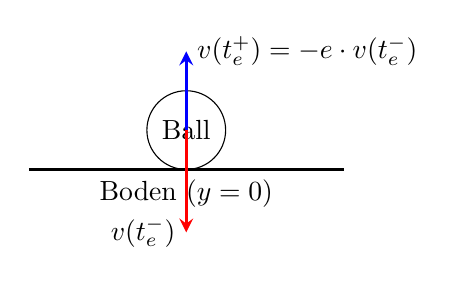
\begin{tikzpicture}[>=stealth]
    % Boden
    \draw[thick] (-2,0) -- (2,0) node[below, midway] {Boden ($y=0$)};

    % Ball
    \draw (0, 0.5) circle (0.5cm);
    \node at (0, 0.5) {Ball};

    % Vektoren
    \draw[->, red, very thick] (0, 0.5) -- (0, -0.8) node[left, black] {$v(t_e^-)$};
    \draw[->, blue, very thick] (0, 0.5) -- (0, 1.5) node[right, black] {$v(t_e^+) = -e \cdot v(t_e^-)$};
\end{tikzpicture}
\end{document}
